%Conclusion body
%Created SS 04-14

\section{Results}
\label{results}

\subsection{Direct Observation}
\subsubsection{$\lambda$-point Transition}
As the temperature of liquid helium was decreased, we witnessed rapid
bubbling of the fluid. The bubbling ceased immediately as the
temperature passed $T_{\lambda}$, confirming the intolerance of helium
II to thermal gradients.

\subsubsection{Fountain Effect}
We observed a small stream of liquid helium emerging from the
capillary of the `fountain' system, described in Section
\ref{superfluidfountain}. The fountain is only visible at temperatures
below the $\lambda$-point, and the height of the stream decreases with
increasing temperature. This provides a good visual demonstration of
the decreasing fraction of superfluid as temperature of the system
approaches $T_{\lambda}$ from below.

\subsection{Second Sound Results}
\label{secondsoundresults}

To measure the velocity of second sound in He II, the propagation time of heat pulses in the superfluid is observed over a range of temperatures. First the displacement between the bolometer and the heater (both fully submerged) is measured. Next, heat pulses sent from the heater propagate towards the bolometer as second sound. The duration between the triggering of the heat pulse and the pulse's signature seen by the bolometer is observed and recorded. Multiple displacements and corresponding durations are recorded for various temperatures ranging from $1.6$ K to $2.2$ K, shown in Fig. \ref{fig:secondsoundraw}. Second sound velocity goes to zero as the temperature approaches $T_{\lambda}$.


\begin{figure}[htbp]
\begin{center}
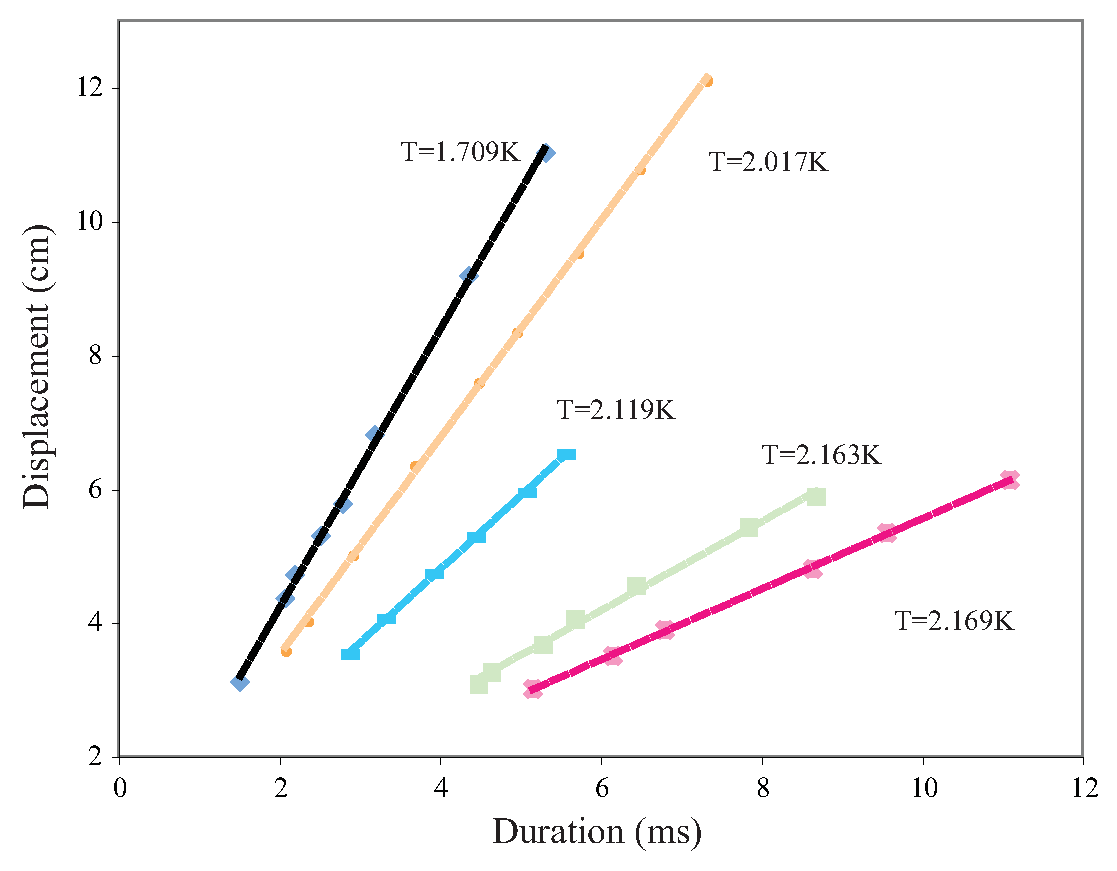
\includegraphics[height=70mm]{./figures/secondsoundraw.eps}
\caption{\small{A plot of the displacement of the thermometer from the heater \emph{versus} the duration between the triggering of the heat pulse and the pulse's signature recorded by the thermometer for various temperatures in He II.}}
\label{fig:secondsoundraw}
\end{center}
\end{figure}


\subsection{Heat Capacity Results}\label{heatcapacityresults}

To measure heat capacity, we observe the effect of heat pulses sent to the cell on a germanium resistor which is thermally coupled to the cell. Beginning at a temperature of about $1.8$ K, $10$ ms heat pulses with a power of $98.8$ mW are sent to the cell.  These heat pulses cause the temperature of the cell to rise which consequently causes the resistance of the coupled germanium resistor to increase.  Because the current through the germanium resistor is a constant $1.00$ $\mu$A, a decrease in resistance causes a decrease in the potential difference across the resistor. The change in the potential difference due to consecutive heat pulses sent to the cell is measured for both the evacuated and filled copper cell. Fig. \ref{fig:rawdata} shows portions of this data for both scenarios.  Over the course of the experimental run, the potential difference in both cases falls in discrete sections due to the consecutive heat pulses. While the changes in potential per heat pulse are uniform in the empty cell for the entire observed temperature range, the changes in potential difference for the filled cell depend upon whether the temperature of the cell is above or below $T_{\lambda}$. This disparity is shown in Fig. \ref{fig:rawdata}. For all data, steady state electric potentials are not completely steady.  Instead, the steady states slightly decrease due to the constant heating of the cell which is not perfectly isolated from the outside environment.

\begin{figure}[htbp]
\begin{center}
\subfigure[Copper cell]{\label{fig:edge-a}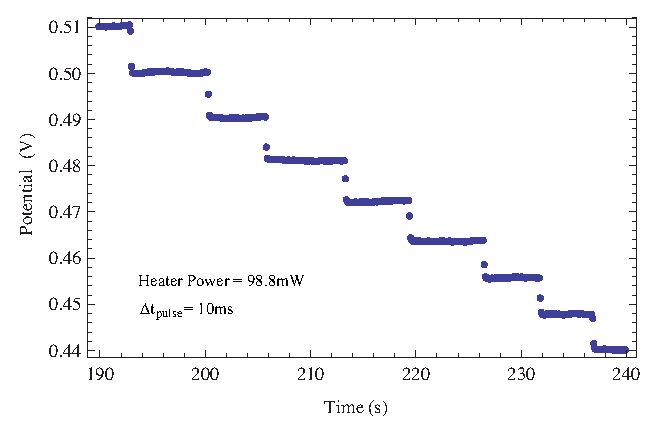
\includegraphics[height=52mm]{figures/rawcu.eps}}
\hspace{-1mm}
\vspace{-2mm}
\subfigure[He II and copper cell near $T_{\lambda}$]{\label{fig:edge-b}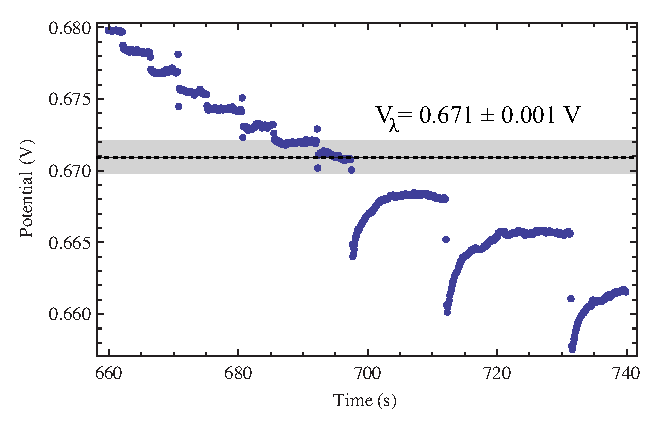
\includegraphics[height=52mm]{figures/rawhe.eps}}
\vspace{-2mm}
\caption{\small{Plots showing the change in the thermometer's potential difference due to heat pulses sent to (a) the evacuated addendum and (b) the addendum filled with He II.  Each heat pulse is $10$ ms with a power of $98.8$ mW.  From this data we see that $T_{\lambda}$ occurs at $0.671 \pm 0.001$ V judging by the sudden change of the heat pulse's signature.}}
\label{fig:rawdata}
\end{center}
\end{figure}

Knowing the amount of energy deposited in the cell along with the change in temperature, we can calculate heat capacity of the evacuated copper cell and the copper cell filled with helium. To calculate the heat capacity of only the helium, we subtract the heat capacity of the evacuated cell from the heat capacity of the filled cell.